\documentclass[11pt,a4paper]{report}
\usepackage[textwidth=37em,vmargin=30mm]{geometry}
\usepackage{calc,xunicode,amsmath,amssymb,paralist,enumitem,tabu,booktabs,datetime2,xeCJK,xeCJKfntef,listings}
\usepackage{tocloft,fancyhdr,tcolorbox,xcolor,graphicx,eso-pic,xltxtra,xelatexemoji}

\newcommand{\envyear}[0]{2025}
\newcommand{\envdatestr}[0]{2025-05-28}
\newcommand{\envfinaldir}[0]{webdb/2025/20250528/final}

\usepackage[hidelinks]{hyperref}
\hypersetup{
    colorlinks=false,
    pdfpagemode=FullScreen,
    pdftitle={Web Digest - \envdatestr}
}

\setlength{\cftbeforechapskip}{10pt}
\renewcommand{\cftchapfont}{\rmfamily\bfseries\large\raggedright}
\setlength{\cftbeforesecskip}{2pt}
\renewcommand{\cftsecfont}{\sffamily\small\raggedright}

\setdefaultleftmargin{2em}{2em}{1em}{1em}{1em}{1em}

\usepackage{xeCJK,xeCJKfntef}
\xeCJKsetup{PunctStyle=plain,RubberPunctSkip=false,CJKglue=\strut\hskip 0pt plus 0.1em minus 0.05em,CJKecglue=\strut\hskip 0.22em plus 0.2em}
\XeTeXlinebreaklocale "zh"
\XeTeXlinebreakskip = 0pt


\setmainfont{Brygada 1918}
\setromanfont{Brygada 1918}
\setsansfont{IBM Plex Sans}
\setmonofont{JetBrains Mono NL}
\setCJKmainfont{Noto Serif CJK SC}
\setCJKromanfont{Noto Serif CJK SC}
\setCJKsansfont{Noto Sans CJK SC}
\setCJKmonofont{Noto Sans CJK SC}

\setlength{\parindent}{0pt}
\setlength{\parskip}{8pt}
\linespread{1.15}

\lstset{
	basicstyle=\ttfamily\footnotesize,
	numbersep=5pt,
	backgroundcolor=\color{black!5},
	showspaces=false,
	showstringspaces=false,
	showtabs=false,
	tabsize=2,
	captionpos=b,
	breaklines=true,
	breakatwhitespace=true,
	breakautoindent=true,
	linewidth=\textwidth
}






\newcommand{\coverpic}[2]{
    % argv: itemurl, authorname
    Cover photo by #2~~(\href{#1}{#1})
}
\newcommand{\makeheader}[0]{
    \begin{titlepage}
        % \newgeometry{hmargin=15mm,tmargin=21mm,bmargin=12mm}
        \begin{center}
            
            \rmfamily\scshape
            \fontspec{BaskervilleF}
            \fontspec{Old Standard}
            \fontsize{59pt}{70pt}\selectfont
            WEB\hfill DIGEST
            
            \vfill
            % \vskip 30pt
            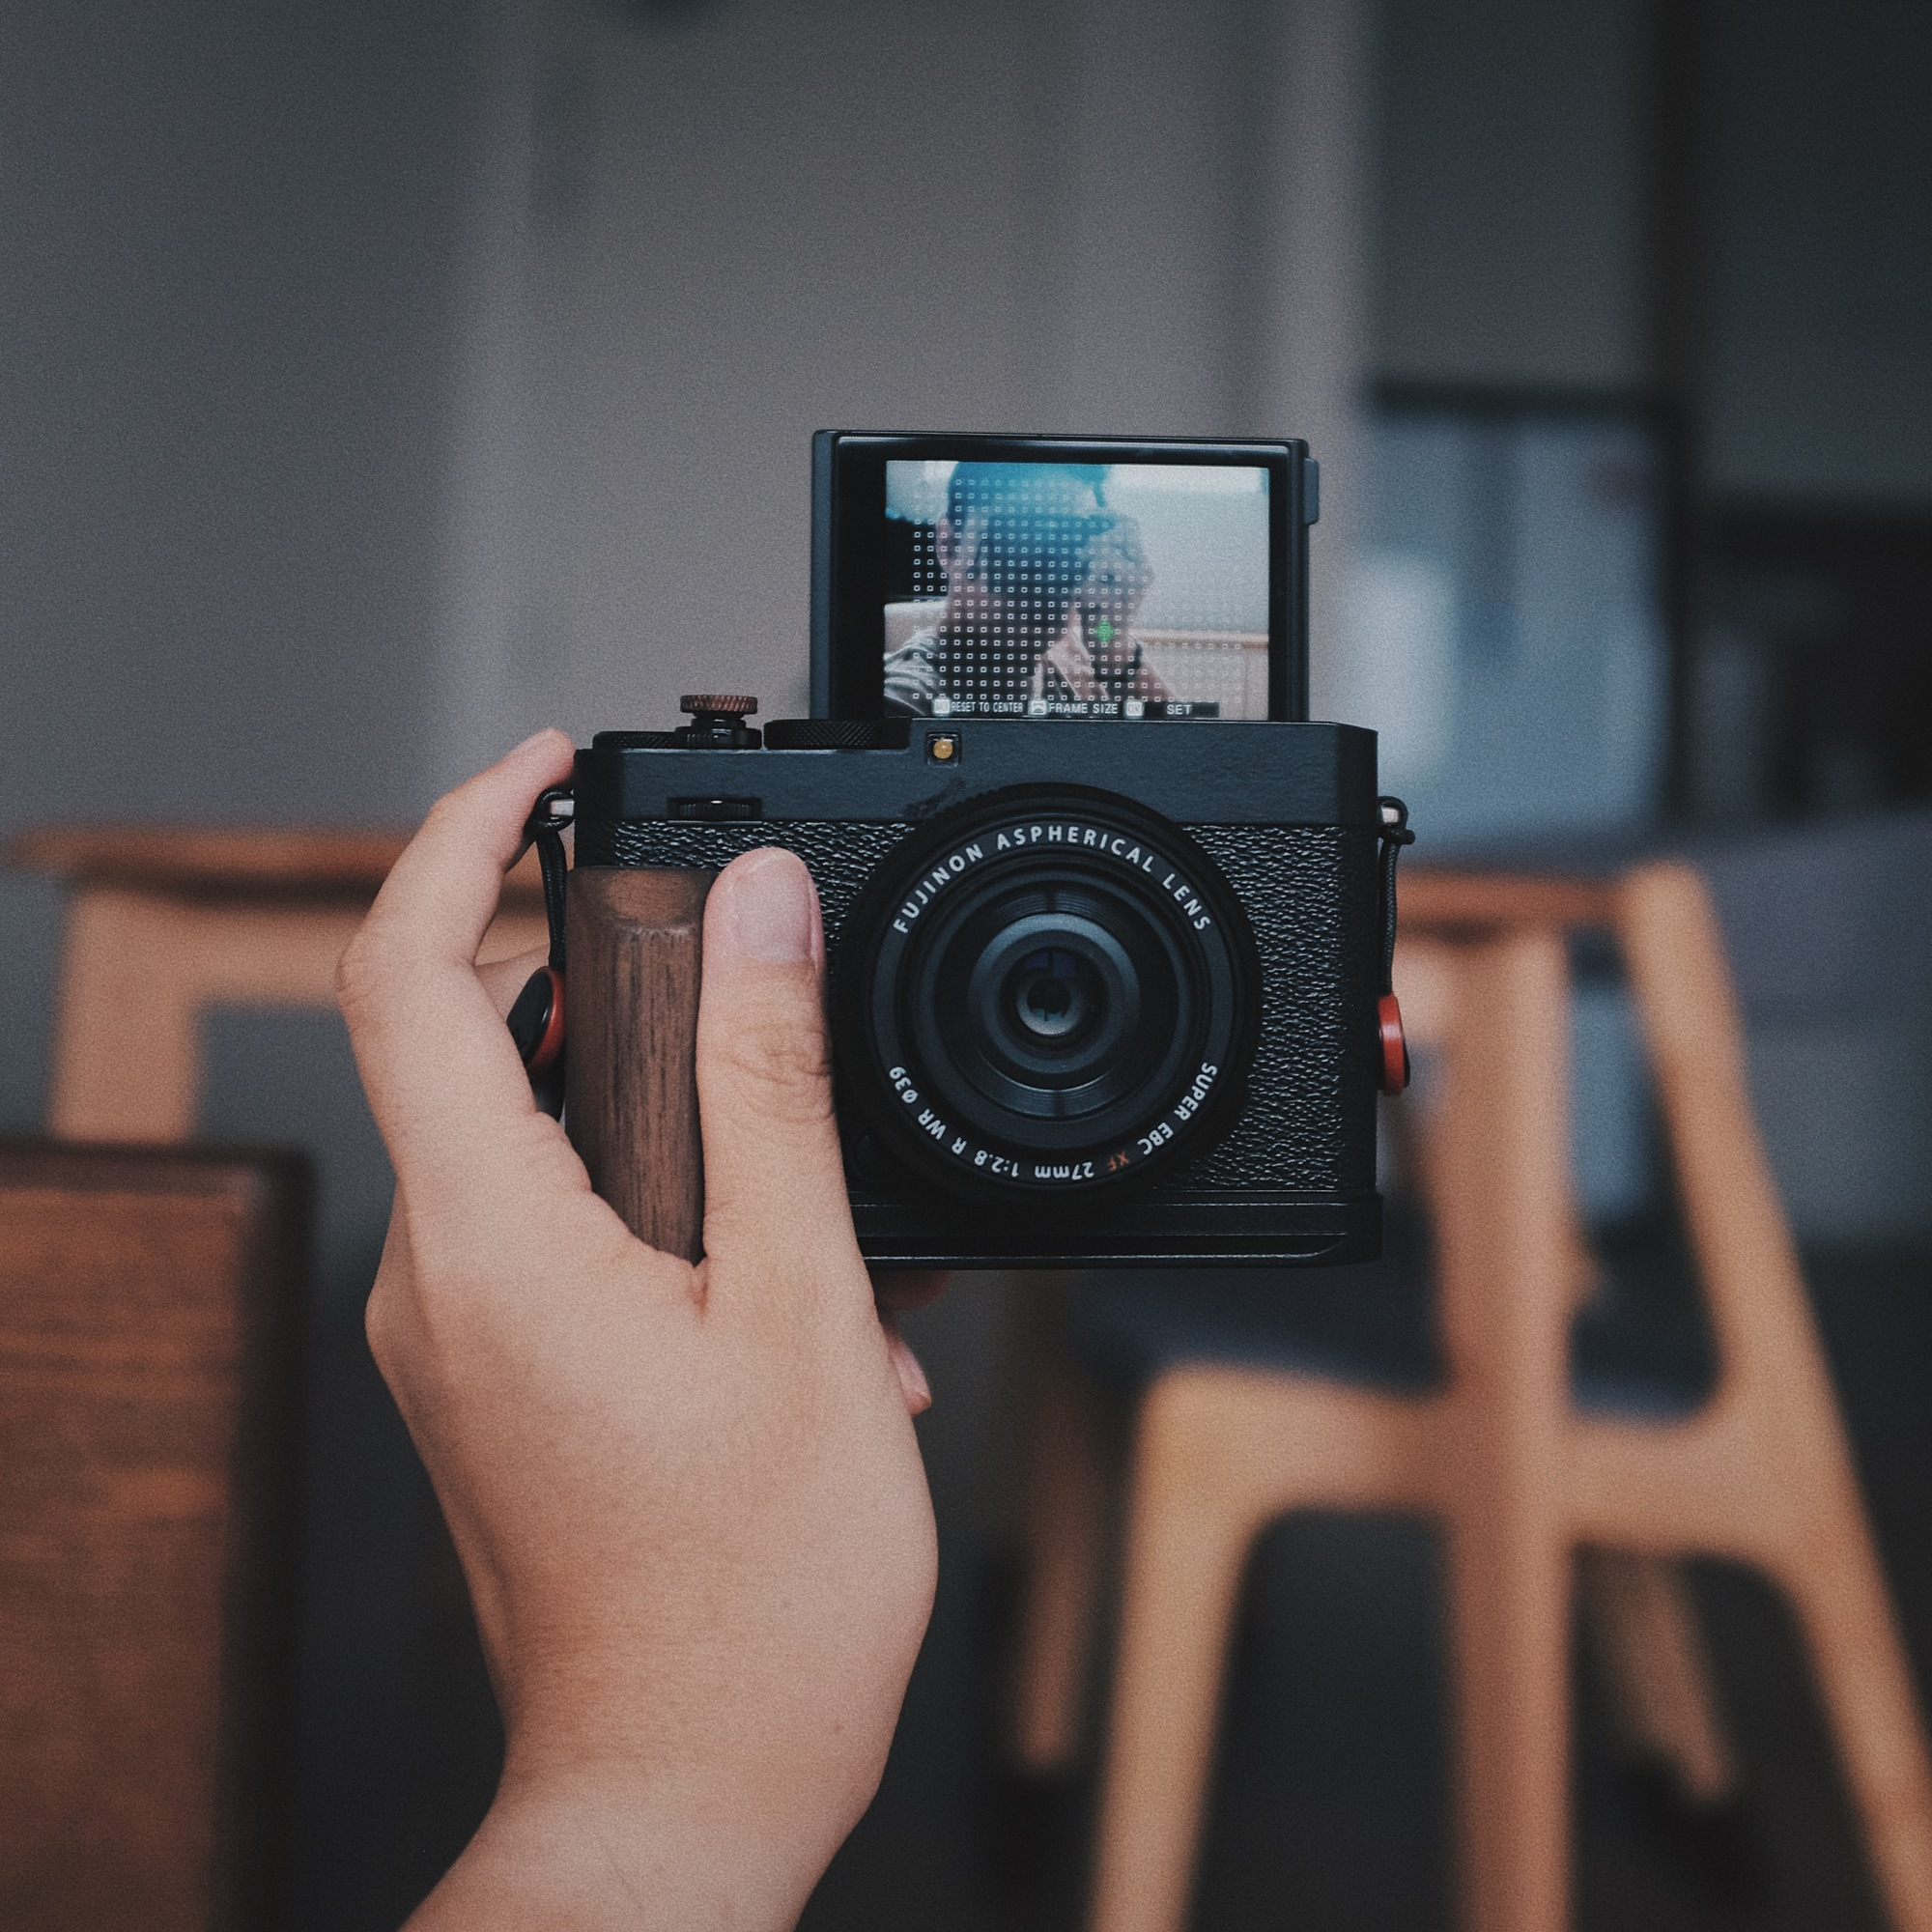
\includegraphics[width=\linewidth]{\envfinaldir/coverpic-prod.jpg}\par
            % \vskip 30pt
            \vfill

            \normalsize\rmfamily\scshape
            \copyright{} The Web Digest Project \hfill\large \envdatestr
        \end{center}
    \end{titlepage}
    % \restoregeometry
}
\newcommand{\simplehref}[1]{%
    \textcolor{blue!80!green}{\href{#1}{#1}}%
}
\renewcommand{\contentsname}{\center\Huge\sffamily\bfseries Contents\par\vskip 20pt}
\newcounter{ipartcounter}
\setcounter{ipartcounter}{0}
\newcommand{\ipart}[1]{
    % \vskip 20pt
    \clearpage
    \stepcounter{ipartcounter}
    \phantomsection
    \addcontentsline{toc}{chapter}{#1}
    % \begin{center}
    %     \Huge
    %     \sffamily\bfseries
    %     #1
    % \end{center}
    % \vskip 20pt plus 7pt
}
\newcounter{ichaptercounter}
\setcounter{ichaptercounter}{0}
\newcommand{\ichapter}[1]{
    % \vskip 20pt
    \clearpage
    \stepcounter{ichaptercounter}
    \phantomsection
    \addcontentsline{toc}{section}{\numberline{\arabic{ichaptercounter}}#1}
    \begin{center}
        \Huge
        \sffamily\bfseries
        #1
    \end{center}
    \vskip 20pt plus 7pt
}
\newcommand{\entrytitlefont}[1]{\subsection*{\raggedright\Large\sffamily\bfseries#1}}
\newcommand{\entryitemGeneric}[2]{
    % argv: title, url
    \parbox{\linewidth}{
        \entrytitlefont{#1}\par\vskip 5pt
        \footnotesize\ttfamily\mdseries
        \simplehref{#2}
    }\vskip 11pt plus 11pt minus 1pt
}
\newcommand{\entryitemGithub}[3]{
    % argv: title, url, desc
    \parbox{\linewidth}{
        \entrytitlefont{#1}\par\vskip 5pt
        \footnotesize\ttfamily\mdseries
        \simplehref{#2}\par\vskip 5pt
        \small\rmfamily\mdseries#3
    }\vskip 11pt plus 11pt minus 1pt
}
\newcommand{\entryitemAp}[3]{
    % argv: title, url, desc
    \parbox{\linewidth}{
        \entrytitlefont{#1}\par\vskip 5pt
        \footnotesize\ttfamily\mdseries
        \simplehref{#2}\par\vskip 5pt
        \small\rmfamily\mdseries#3
    }\vskip 11pt plus 11pt minus 1pt
}
\newcommand{\entryitemHackernews}[3]{
    % argv: title, hnurl, rawurl
    % \parbox{\linewidth}{
    %     \entrytitlefont{#1}\par\vskip 5pt
    %     \footnotesize\ttfamily\mdseries
    %     \simplehref{#3}\par
    %     \textcolor{black!50}{\href{#2}{#2}}
    % }\vskip 11pt plus 11pt minus 1pt
    \begin{minipage}{\linewidth}
            \entrytitlefont{#1}\par\vskip 5pt
            \footnotesize\ttfamily\mdseries
            \simplehref{#3}\par
            \textcolor{black!50}{\href{#2}{#2}}
    \end{minipage}\par\vskip 11pt plus 11pt minus 1pt
}







\begin{document}

\makeheader

\tableofcontents\clearpage




\ipart{Developers}
\ichapter{Hacker News}
\entryitemTwoLinks{Show HN: My LLM CLI tool can run tools now, from Python code or plugins}{https://news.ycombinator.com/item?id=44110584}{https://simonwillison.net/2025/May/27/llm-tools/}

\entryitemTwoLinks{Why the Original Macintosh Had a Screen Resolution of 512×324}{https://news.ycombinator.com/item?id=44110219}{https://512pixels.net/2025/05/original-macintosh-resolution/}

\entryitemTwoLinks{US pauses new student visa interviews as it mulls expanding social media vetting}{https://news.ycombinator.com/item?id=44109253}{https://www.politico.com/news/2025/05/27/trump-team-orders-stop-to-new-student-visa-interviews-as-it-weighs-expanding-social-media-vetting-00370501}

\entryitemTwoLinks{I salvaged \$6k of luxury items discarded by Duke students}{https://news.ycombinator.com/item?id=44108207}{https://indyweek.com/culture/duke-students-dumpster-diving/}

\entryitemTwoLinks{Square Theory}{https://news.ycombinator.com/item?id=44107942}{https://aaronson.org/blog/square-theory}

\entryitemTwoLinks{Pyrefly vs. Ty: Comparing Python's two new Rust-based type checkers}{https://news.ycombinator.com/item?id=44107655}{https://blog.edward-li.com/tech/comparing-pyrefly-vs-ty/}

\entryitemTwoLinks{Mistral Agents API}{https://news.ycombinator.com/item?id=44107187}{https://mistral.ai/news/agents-api}

\entryitemTwoLinks{Why Cline doesn't index your codebase}{https://news.ycombinator.com/item?id=44106944}{https://cline.bot/blog/why-cline-doesnt-index-your-codebase-and-why-thats-a-good-thing}

\entryitemTwoLinks{DuckLake is an integrated data lake and catalog format}{https://news.ycombinator.com/item?id=44106934}{https://ducklake.select/}

\entryitemTwoLinks{How a hawk learned to use traffic signals to hunt more successfully}{https://news.ycombinator.com/item?id=44105965}{https://www.frontiersin.org/news/2025/05/23/street-smarts-hawk-use-traffic-signals-hunting}

\entryitemTwoLinks{Just make it scale: An Aurora DSQL story}{https://news.ycombinator.com/item?id=44105878}{https://www.allthingsdistributed.com/2025/05/just-make-it-scale-an-aurora-dsql-story.html}

\entryitemTwoLinks{BGP handling bug causes widespread internet routing instability}{https://news.ycombinator.com/item?id=44105796}{https://blog.benjojo.co.uk/post/bgp-attr-40-junos-arista-session-reset-incident}

\entryitemTwoLinks{LumoSQL}{https://news.ycombinator.com/item?id=44105619}{https://lumosql.org/src/lumosql/doc/trunk/README.md}

\entryitemTwoLinks{The Myth of Developer Obsolescence}{https://news.ycombinator.com/item?id=44105592}{https://alonso.network/the-recurring-cycle-of-developer-replacement-hype/}

\entryitemTwoLinks{Revisiting the algorithm that changed horse race betting (2023)}{https://news.ycombinator.com/item?id=44105470}{https://actamachina.com/posts/annotated-benter-paper}

\entryitemTwoLinks{LiveStore: State management based on reactive SQLite and built-in sync engine}{https://news.ycombinator.com/item?id=44105412}{https://livestore.dev}

\entryitemTwoLinks{Show HN: Lazy Tetris}{https://news.ycombinator.com/item?id=44103839}{https://lazytetris.com/}

\entryitemTwoLinks{The UI future is colourful and dimensional}{https://news.ycombinator.com/item?id=44103131}{https://www.flarup.email/p/the-future-is-colourful-and-dimensional}

\entryitemTwoLinks{Yes-rs: A fast, memory-safe rewrite of the classic Unix yes command}{https://news.ycombinator.com/item?id=44103116}{https://github.com/jedisct1/yes-rs}

\entryitemTwoLinks{Calendars, Contacts and Files in Stalwart}{https://news.ycombinator.com/item?id=44103071}{https://stalw.art/blog/collaboration/}\ichapter{Phoronix}
\entryitemGeneric{\hskip 0pt{}Linux 6.16 Upstreams Support For Hardware-Wrapped Encryption Keys}{https://www.phoronix.com/news/Linux-6.16-FSCRYPT-Wrapped-Keys}

\entryitemGeneric{\hskip 0pt{}Intel APX Ready With Linux 6.16, Outdated Intel CPU Microcode Reporting Merged}{https://www.phoronix.com/news/Linux-6.16-x86-Core}

\entryitemGeneric{\hskip 0pt{}AlmaLinux 10.0 Stable Released - Unlike RHEL 10, It Continues Supporting x86-64-v2 CPUs}{https://www.phoronix.com/news/AlmaLinux-10.0-Released}

\entryitemGeneric{\hskip 0pt{}Wayland ext-background-effect-v1 Merged For Background Blur Feature}{https://www.phoronix.com/news/Wayland-Background-Effect}

\entryitemGeneric{\hskip 0pt{}ROCm GPU Compute Performance With AMD Ryzen AI MAX+ "Strix Halo"}{https://www.phoronix.com/review/amd-strix-halo-rocm-benchmarks}

\entryitemGeneric{\hskip 0pt{}XFS Atomic Writes Support Merged For Linux 6.16}{https://www.phoronix.com/news/XFS-Atomic-Writes-Linux-6.16}

\entryitemGeneric{\hskip 0pt{}Linux 6.16 Adds "X86\_NATIVE\_CPU" Option To Optimize Your Kernel Build For Your CPU}{https://www.phoronix.com/news/Linux-6.16-X86\_NATIVE\_CPU}

\entryitemGeneric{\hskip 0pt{}Rav1e v0.8 Released For Rust-Based AV1 Encoding}{https://www.phoronix.com/news/Rav1e-0.8-Released}

\entryitemGeneric{\hskip 0pt{}Linux 6.16 Lands "rt\_group\_sched" Option, Faster Core Offlining \& Scheduler Improvements}{https://www.phoronix.com/news/Linux-6.16-Scheduler}\ichapter{Dribbble}
\entryitemGeneric{\hskip 0pt{}Credit payment card bank app animation}{https://dribbble.com/shots/26063214-Credit-payment-card-bank-app-animation}

\entryitemGeneric{\hskip 0pt{}HYDRO - Logo Design}{https://dribbble.com/shots/26073470-HYDRO-Logo-Design}

\entryitemGeneric{\hskip 0pt{}Project Management Dashboard}{https://dribbble.com/shots/26070177-Project-Management-Dashboard}

\entryitemGeneric{\hskip 0pt{}Stanley // Website}{https://dribbble.com/shots/26056691-Stanley-Website}

\entryitemGeneric{\hskip 0pt{}AltSocial}{https://dribbble.com/shots/26060858-AltSocial}

\entryitemGeneric{\hskip 0pt{}i SEA you}{https://dribbble.com/shots/26062936-i-SEA-you}

\entryitemGeneric{\hskip 0pt{}Fariland Headwear Symbol}{https://dribbble.com/shots/26063219-Fariland-Headwear-Symbol}

\entryitemGeneric{\hskip 0pt{}Glassmorphic 3D Logo Animation}{https://dribbble.com/shots/26061835-Glassmorphic-3D-Logo-Animation}

\entryitemGeneric{\hskip 0pt{}Meditation App Branding Concept}{https://dribbble.com/shots/26057810-Meditation-App-Branding-Concept}

\entryitemGeneric{\hskip 0pt{}Landing Page for an AI-Powered Design System}{https://dribbble.com/shots/26057663-Landing-Page-for-an-AI-Powered-Design-System}

\entryitemGeneric{\hskip 0pt{}Medic H - Logo Design}{https://dribbble.com/shots/26057472-Medic-H-Logo-Design}

\entryitemGeneric{\hskip 0pt{}Smart Home App}{https://dribbble.com/shots/26056748-Smart-Home-App}

\entryitemGeneric{\hskip 0pt{}Sellin dashboard}{https://dribbble.com/shots/26037015-Sellin-dashboard}

\entryitemGeneric{\hskip 0pt{}Fariland Headwear}{https://dribbble.com/shots/26058705-Fariland-Headwear}

\entryitemGeneric{\hskip 0pt{}Travel Startup Branding for Holidu: visual identity brand design}{https://dribbble.com/shots/25983747-Travel-Startup-Branding-for-Holidu-visual-identity-brand-design}

\entryitemGeneric{\hskip 0pt{}Illustration}{https://dribbble.com/shots/26052539-Illustration}

\entryitemGeneric{\hskip 0pt{}Playground web interaction}{https://dribbble.com/shots/26048246-Playground-web-interaction}

\entryitemGeneric{\hskip 0pt{}Onday - Logo Design}{https://dribbble.com/shots/26053436-Onday-Logo-Design}

\entryitemGeneric{\hskip 0pt{}Burger Time!}{https://dribbble.com/shots/26053795-Burger-Time}

\entryitemGeneric{\hskip 0pt{}Homepage Design — WoodNest}{https://dribbble.com/shots/26051400-Homepage-Design-WoodNest}

\entryitemGeneric{\hskip 0pt{}Mighty Sketches}{https://dribbble.com/shots/26034483-Mighty-Sketches}

\entryitemGeneric{\hskip 0pt{}Magus Brand Identity Design}{https://dribbble.com/shots/26052344-Magus-Brand-Identity-Design}

\entryitemGeneric{\hskip 0pt{}Album}{https://dribbble.com/shots/26050401-Album}

\entryitemGeneric{\hskip 0pt{}Indonesia Travel Poster}{https://dribbble.com/shots/26049146-Indonesia-Travel-Poster}


\ipart{Developers~~~~(zh-Hans)}
\ichapter{Solidot}
\entryitemGeneric{\hskip 0pt{}银河系的一根``骨骼''被脉冲星撞断}{https://www.solidot.org/story?sid=81409}

\entryitemGeneric{\hskip 0pt{}The Browser Company 停止开发 Arc 转向 AI 驱动浏览器 Dia }{https://www.solidot.org/story?sid=81408}

\entryitemGeneric{\hskip 0pt{}AI 模型出现崩溃迹象}{https://www.solidot.org/story?sid=81407}

\entryitemGeneric{\hskip 0pt{}BGP 系统的 Bug 处理方式导致部分网络故障}{https://www.solidot.org/story?sid=81406}

\entryitemGeneric{\hskip 0pt{}鹰利用交通灯捕猎}{https://www.solidot.org/story?sid=81405}

\entryitemGeneric{\hskip 0pt{}腾讯将成为 K-Pop 经纪公司 SM娱乐的第二大股东}{https://www.solidot.org/story?sid=81404}

\entryitemGeneric{\hskip 0pt{}台积电下注基于 MicroLED 的光互联技术}{https://www.solidot.org/story?sid=81403}

\entryitemGeneric{\hskip 0pt{}金星共轨小行星可能威胁到地球}{https://www.solidot.org/story?sid=81402}

\entryitemGeneric{\hskip 0pt{}CIA 曾经秘密运营了一家星球大战粉丝网站}{https://www.solidot.org/story?sid=81401}

\entryitemGeneric{\hskip 0pt{}巴基斯坦分配 2000 MW 电力用于挖掘比特币和 AI 数据中心}{https://www.solidot.org/story?sid=81400}

\entryitemGeneric{\hskip 0pt{}普京表态要封锁微软和 Zoom 的服务}{https://www.solidot.org/story?sid=81399}

\entryitemGeneric{\hskip 0pt{}四名大众前高管因柴油门排放丑闻被判刑}{https://www.solidot.org/story?sid=81398}

\entryitemGeneric{\hskip 0pt{}Firefox 139.0 释出}{https://www.solidot.org/story?sid=81397}

\entryitemGeneric{\hskip 0pt{}新材料被动从空气中收集水分}{https://www.solidot.org/story?sid=81396}

\entryitemGeneric{\hskip 0pt{}SerenityOS 创始人开发自己的独立浏览器 Ladybird}{https://www.solidot.org/story?sid=81395}

\entryitemGeneric{\hskip 0pt{}世界是否需要公有社交网络}{https://www.solidot.org/story?sid=81394}

\entryitemGeneric{\hskip 0pt{}英伟达准备推出新款中国专用 AI 芯片}{https://www.solidot.org/story?sid=81393}

\entryitemGeneric{\hskip 0pt{}木星早期大小是目前的两倍}{https://www.solidot.org/story?sid=81392}

\entryitemGeneric{\hskip 0pt{}天文学家发现黏在一起的双星}{https://www.solidot.org/story?sid=81391}

\entryitemGeneric{\hskip 0pt{}亚马逊程序员感觉他们开始像从事仓库工作的流水线工人}{https://www.solidot.org/story?sid=81390}\ichapter{V2EX}
\entryitemGeneric{\hskip 0pt{}[问与答] cursor 长时间使用后变卡}{https://www.v2ex.com/t/1134764}

\entryitemGeneric{\hskip 0pt{}[Go 编程语言] 关于 GO 语言字母与数字交叉打印的问题}{https://www.v2ex.com/t/1134763}

\entryitemGeneric{\hskip 0pt{}[问与答] 裁员, n 走人还是坚持 n+1}{https://www.v2ex.com/t/1134762}

\entryitemGeneric{\hskip 0pt{}[反馈] 请求增加赞助支付方式 ko-fi 使用受阻}{https://www.v2ex.com/t/1134761}

\entryitemGeneric{\hskip 0pt{}[分享创造] 开源的单机游戏变速器,突破游戏帧率限制}{https://www.v2ex.com/t/1134760}

\entryitemGeneric{\hskip 0pt{}[问与答] WhatsApp 注册的电话卡推荐}{https://www.v2ex.com/t/1134758}

\entryitemGeneric{\hskip 0pt{}[程序员] B 站 漏洞 可查询 IP 和设备精确到型号}{https://www.v2ex.com/t/1134757}

\entryitemGeneric{\hskip 0pt{}[信息安全] 网络流量处理中的协议解析一:流量处理模型}{https://www.v2ex.com/t/1134756}

\entryitemGeneric{\hskip 0pt{}[移民] 关于美国签证申请}{https://www.v2ex.com/t/1134755}

\entryitemGeneric{\hskip 0pt{}[问与答] 选择 React-native 的一些理由}{https://www.v2ex.com/t/1134754}

\entryitemGeneric{\hskip 0pt{}[Apple] iPad 怎么这么挑充电头/充电线呢?}{https://www.v2ex.com/t/1134753}

\entryitemGeneric{\hskip 0pt{}[宽带症候群] tailscale 自部署的基于 IP 的中继服务器是否安全?}{https://www.v2ex.com/t/1134752}

\entryitemGeneric{\hskip 0pt{}[酷工作] Java 自动化-上海/成都, 1000-1500/天, 3 天 onsite2 天在家办公}{https://www.v2ex.com/t/1134750}

\entryitemGeneric{\hskip 0pt{}[问与答] 咸鱼的厂家直销靠谱吗}{https://www.v2ex.com/t/1134748}

\entryitemGeneric{\hskip 0pt{}[微信] 现在无论是 iOS 版还是 Android 版,在启动微信小程序直播画面之前,都 TM 给你加上了广告,吃香难看!}{https://www.v2ex.com/t/1134746}

\entryitemGeneric{\hskip 0pt{}[iPhone] 关于 FaceTime 成灰色的疑问}{https://www.v2ex.com/t/1134743}

\entryitemGeneric{\hskip 0pt{}[前端开发] 什么值得买的资讯中心,点击一篇报道之后返回,总是回到页面最上面}{https://www.v2ex.com/t/1134742}

\entryitemGeneric{\hskip 0pt{}[问与答] 前几天看到坛友发文要注意耳朵失聪风险,今天检查完喜忧参半}{https://www.v2ex.com/t/1134740}

\entryitemGeneric{\hskip 0pt{}[程序员] 翻译了 PatrickJS/awesome-cursorrules}{https://www.v2ex.com/t/1134739}

\entryitemGeneric{\hskip 0pt{}[程序员] TRAE 国际版 PRO 版本来了,收费\$10 一个月}{https://www.v2ex.com/t/1134738}

\entryitemGeneric{\hskip 0pt{}[酷工作] 深圳/海外游戏推荐平台项目,招产品经理}{https://www.v2ex.com/t/1134737}

\entryitemGeneric{\hskip 0pt{}[问与答] 有老哥用过西非那地片吗?}{https://www.v2ex.com/t/1134736}

\entryitemGeneric{\hskip 0pt{}[问与答] Windows 11 上, Kafka 客户端每次连接 Kafka,有很大几率卡在 Inet6AddressImpl 的 native 方法 getHostByAddr 上 5 秒}{https://www.v2ex.com/t/1134735}

\entryitemGeneric{\hskip 0pt{}[分享创造] 我开发了一个面向大语言模型的智能数据集构建工具}{https://www.v2ex.com/t/1134733}

\entryitemGeneric{\hskip 0pt{}[生活] 回首过去 32 年,全是痛苦、遗憾、懊悔……}{https://www.v2ex.com/t/1134732}

\entryitemGeneric{\hskip 0pt{}[骑行] 发现还有线控升降座杆这种产品,真心请教下, 单车算比较私人的运动工具,快速调节还不够用?}{https://www.v2ex.com/t/1134731}

\entryitemGeneric{\hskip 0pt{}[程序员] 国际版 Trae 开始收费了}{https://www.v2ex.com/t/1134730}

\entryitemGeneric{\hskip 0pt{}[分享发现] 第一次发现一首在百度都搜不到的歌}{https://www.v2ex.com/t/1134729}

\entryitemGeneric{\hskip 0pt{}[问与答] todesk 太恶心了}{https://www.v2ex.com/t/1134727}

\entryitemGeneric{\hskip 0pt{}[酷工作] base 深圳内推 IOS、 Java 、Go、web(H5)前端研发岗,流程快}{https://www.v2ex.com/t/1134726}

\entryitemGeneric{\hskip 0pt{}[问与答] 武汉某马公司面试,疑似偷方案,可以直接开喷吗?}{https://www.v2ex.com/t/1134724}

\entryitemGeneric{\hskip 0pt{}[云计算] 618 国内主机商有活动吗?}{https://www.v2ex.com/t/1134723}

\entryitemGeneric{\hskip 0pt{}[分享发现] 找到一个和大模型有意思的对话,关于机器人的,哈哈哈}{https://www.v2ex.com/t/1134722}

\entryitemGeneric{\hskip 0pt{}[汽车] 谁是汽车圈的``恒大''?}{https://www.v2ex.com/t/1134721}

\entryitemGeneric{\hskip 0pt{}[互联网] QQ 音乐是穷疯了吗?无处不在的牛皮癣}{https://www.v2ex.com/t/1134720}

\entryitemGeneric{\hskip 0pt{}[Linux] Linux 如何找出本地 DNS 请求来源}{https://www.v2ex.com/t/1134719}

\entryitemGeneric{\hskip 0pt{}[程序员] 客户端研发上手后端需要几天?}{https://www.v2ex.com/t/1134718}

\entryitemGeneric{\hskip 0pt{}[问与答] 关于减肥饮食记录软件}{https://www.v2ex.com/t/1134717}

\entryitemGeneric{\hskip 0pt{}[Apple] 问下,目前苹果系统的家庭、照片、日程等 app 还会收到垃圾消息吗?}{https://www.v2ex.com/t/1134716}

\entryitemGeneric{\hskip 0pt{}[Amazon Web Services] 来一个 AWS 的销售联系方式}{https://www.v2ex.com/t/1134715}

\entryitemGeneric{\hskip 0pt{}[全球工单系统] 腾讯微云要倒闭了吗?短信验证码一直收不到}{https://www.v2ex.com/t/1134714}

\entryitemGeneric{\hskip 0pt{}[Apple] 24 寸 4K 是不是伪命题?}{https://www.v2ex.com/t/1134713}

\entryitemGeneric{\hskip 0pt{}[分享发现] 单座 eVTOL 飞行器 (个人飞行摩托) 市场调研问卷, 欢迎来填}{https://www.v2ex.com/t/1134711}

\entryitemGeneric{\hskip 0pt{}[程序员] deepseek+ollama+disy 部署收多少}{https://www.v2ex.com/t/1134710}

\entryitemGeneric{\hskip 0pt{}[iOS] 请教一下, ios 系统如何升级到指定版本,大版本就行,如果可以精确到小版本也行}{https://www.v2ex.com/t/1134709}

\entryitemGeneric{\hskip 0pt{}[汽车] 预算 30w 可以考虑 A6L 么}{https://www.v2ex.com/t/1134707}

\entryitemGeneric{\hskip 0pt{}[程序员] Java 如何使用 cursor 开发}{https://www.v2ex.com/t/1134706}

\entryitemGeneric{\hskip 0pt{}[问与答] Adobe 订阅推荐,马上到期了,求推荐!}{https://www.v2ex.com/t/1134705}

\entryitemGeneric{\hskip 0pt{}[杭州] 端午节杭州周边遛娃有推荐吗}{https://www.v2ex.com/t/1134704}

\entryitemGeneric{\hskip 0pt{}[云计算] [阿里云] 关于电信运营商禁止短信内容包含链接、IP 地址、联系方式的公告}{https://www.v2ex.com/t/1134702}


\ipart{Generic News}







\clearpage
\leavevmode\vfill
\footnotesize

Copyright \copyright{} 2023-2025 Neruthes and other contributors.

This document is published with CC BY-NC-ND 4.0 license.

The entries listed in this newsletter may be copyrighted by their respective creators.

This newsletter is generated by the Web Digest project.

The newsletters are also delivered via Telegram channel \CJKunderline{\href{https://t.me/webdigestchannel}{https://t.me/webdigestchannel}}.\\
RSS feed is available at \CJKunderline{\href{https://webdigest.pages.dev/rss.xml}{https://webdigest.pages.dev/rss.xml}}.

This newsletter is available in PDF at
\CJKunderline{\href{https://webdigest.pages.dev/}{https://webdigest.pages.dev/}}.

The source code being used to generate this newsletter is available at\\
\CJKunderline{\href{https://github.com/neruthes/webdigest}{https://github.com/neruthes/webdigest}}.

This newsletter is also available in
\CJKunderline{\href{http://webdigest.pages.dev/readhtml/\envyear/WebDigest-20250528.html}{HTML}} and
\CJKunderline{\href{https://github.com/neruthes/webdigest/blob/master/markdown/\envyear/WebDigest-20250528.md}{Markdown}}.


\coverpic{https://unsplash.com/photos/a-close-up-of-a-green-porsche-911-PLjANvI6Jtk}{Dmitry Spravko}


\end{document}
